
\chapter{자기주도적 학습 과제 2 (12.5-6)}

\section{$\mathbb{R}^3$에서 거리 구하는 공식 만들고 $n$차원 확장}

$p _{0} + q _{0} t$과  $p _{1} + q _{1} t$ 생각하자

\paragraph{3차원에서의 거리공식}
두 직선이 만드는 평면의 법선벡터를 생각한다. 직선 위 임의의 두 점을 잇는 벡터를, 
이 법선벡터에 사영시킨 것이 바로 거리가 될 것이다.

$\left| \mathrm{proj} _{q _1 \times  q _{2}} ( p _{1} - p _{2} ) \right|$

\paragraph{$n$차원 확장 방법 1}

해가 존재한다면, $q_0$, $q_1$은 평행하지 않다.
$q_0$, $q_1$, $p_0 - p_1$을 세 기저로 하는 공간을 생각할 수 있고,
만일 그렇다면, 나머지 기저들은 거리 공식에 영향을 다 못 줄 것(싹 다 0임). 
이 기저들을, 가우스-조르단 방법 하듯이 하듯 잘 손질하면 
수직인 세 백터로 만들 수 있을 것이고, 그러면 3차원 백터가 나오니까 위의 공식에 대입한다!

\paragraph{$n$차원 확장 방법 2}
2학년 1학기 일반물리학 실험때 배운 최소제곱법 유도방식을 이용하자.

저 두 직선을 빼면, $a+bs+ct$꼴이며, 거리의 제곱을 구하면, $\sum \left( a(n) + b(n)s + c(n) t \right)^2 $이며,
$s$와 $t$에 각각 편미분 해주면, 2원 1차 연립방정식의 꼴이 된다. 따라서, 
$\begin{bmatrix} s \\t \end{bmatrix}$ $ =- \begin{bmatrix} \Sigma  ab \\ \Sigma  ac  \end{bmatrix} \begin{bmatrix} \Sigma  b ^{2}& \Sigma  bc \\ \Sigma  bc& \Sigma  c ^{2} \end{bmatrix}  ^{-1} $로 어떤 값을 구할 수 있으며, 거리는 와 가 무한하면 무한하며, 대충 아래로 볼록한 이차식 형태꼴로 나오는 것으로 예상되며, 저 값이 최소값이라고 추측된다.
따라서, 저 $s$와 $t$를 대입한 거리값이 최소값일 가능성이 매우 높다.


\section{곡선의 정의}

\paragraph{위키피디아 정의}  

연속적인 점들의 집합이다.

구간 $I$와 위상공간 $X$가 있을 때, $I \to X$의 연속함수
\paragraph{위상공간} 
어떤 점의 근처(근방)가 무엇인지에 대한 정보를 담고 있지만, 점 사이의 거리나 넓이·부피 따위의 정보를 포함하지 않는 공간.

\paragraph{근방}
어떤 점의 주위를 포함하는 집합. 위상공간 $X$속 점 $x \in X$의 근방은 $x$를 원소로 포함하는 열린 부분집합이다.

\paragraph{선생님 PPT}
사상 $\left[ a, b\right] \Rightarrow \mathbb{R}^n$에 대해, $t$가 $\left[ a, b\right]$에서 변할 때, 점들의 모임
\section{페아노 곡선의 정의와 성질}

\begin{figure}[h!]
    \centering
    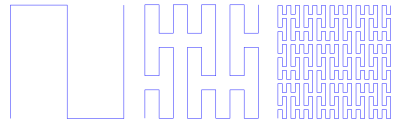
\includegraphics[width=.7\textwidth]{img/peano.png  }
    \caption{페아노 곡선의 모습}
    \label{texlive:exdit}
\end{figure}

자연수를 정의하여 수많은 수학덕을 양성(?)한 것으로 유명한 이탈리아 수학자 주세페 페아노가 1980에 발견한 곡선이다. 
단위 길이를 단위 평면에 대응시키는 전사 함수이다. 
칸토어가 $\mathrm{Card}(N)=\mathrm{Card}(N ^{2})$ 증명하는데 영감을 줬다고 한다.
공간충전곡선(空間充塡曲線)의 한 예이며, 교점 없이 평면공간, 더 나아가 임의의 폐집합 내를 체우는 곡선이다. 


\section{타원면과 만나는 평면의 방향과는 상관 없이 교차하는 부분은 타원인가}

중명 1.
$x ^{2} /a ^{2} +y ^{2} /b ^{2} +z ^{2} /c ^{2} =1$과, $a' x+b' y+c' z=d$ 두 선의 교점이라고 생각하자. 평면의 식을 $z$에 대해 정리한 뒤, 첫 번째 공식에 대입하게 되면, $x^2$, $y^2$, $x$, $y$등이 담긴 방정식이 나온다. 근데, 
\begin{enumerate}
    \item  $x^2$과 $y^2$의 부호가 같을 것이 자명하다. 
    \item 타원의 경우 정의역이 제한되어 있기 때문에, 결과 식도 어느 범위로 재한되어 있으며, 이를 만족하는 이차함수는 타원이 유일하니까
\end{enumerate}
$\to$ 결과는 타원이다.

이는 교선을 $xy$평면에 사영시킨 것인데, 원래 교선도 어떤 평면 위에 있으니까,
$xy$평면에서 거리에 관한 공식들이, 어떤 평면과 $xy$평면의 이면각 $\theta$에 대해, $\cos(\theta)$에 비례하는 형태를 띄게 된다. 
따라서, 두 초점 사이 거리 관계가 $xy$평면에서 성립하면, 원래 평면에서도 성립하므로, 원래 평면에서 그려진 교선은 타원이다.

\section{카발리에리의 원리로 타원면으로 둘러싸인 부분의 부피 구하는 공식을 만들기. 그리고 $n$차원으로 확장하시오.}
타원 면적 구하는 공식은 $\pi a b$이다.

타원면을  $ \frac{x ^2}{a^2} +\frac{y^2}{b^2} + \frac{z^2}{c^2} =1$로 잡자.

$z=z$인 평면을 기준으로 생각하면, $1 - \frac{z ^{2}}{c^2} = \frac{x ^2}{a^2} +\frac{y^2}{b^2}  $이니, 면적은 $\pi ab \sqrt {1-z ^{2}}$이다.

이는 $\pi \sqrt {1-z ^{2}}$를 $ab$배 한 것이니, 
구하구자 하는 부피는 카빌리에리 원리에 의해 $1- \frac{z^2}{c^2} =x ^{2} +y ^{2}$ 의 부피의 $ab$배 일 것이다.
이걸 $-c$부터 $+c$까지 적분하면 $\frac{4}{3}\pi c$이며, 따라서 타원면의 면적은 $\frac{4}{3}\pi abc$이다.